\documentclass[aspectratio=169]{beamer}
\usepackage{ices}
\renewcommand\r[1]{\textblue{#1}}
\title{ICES Web Services and R}
\author{Colin Millar\\[0.5ex]Arni Magnusson}
\date{ICES, 3 November 2016}
\begin{document}

\begin{frame}
  \titlepage
\end{frame}

\begin{frame}{Outline}\small
  \textbf{ICES web services}\\[-1ex]
  \begin{itemize}
    \item[-] Data
    \item[-] Formats\\[4ex]
  \end{itemize}
  \textbf{R}\\[-1.5ex]
  \begin{itemize}
    \item[-] Read data
    \item[-] Packages\\[4.5ex]
  \end{itemize}
  \textbf{Discussion}\\[-1ex]
  \begin{itemize}
    \item[-] Standardizing ICES web services
    \item[-] Other topics\\[3ex]
  \end{itemize}
\end{frame}

% ______________________________________________________________________________

\begin{frame}{Web services}\small
  {\green What are web services?}\\[-1ex]
  \begin{itemize}\footnotesize
    \item[] Web services run on the web and allow one application to\\
    speak to another without the need for pressing a button\\[1.5ex]
    \item[] Special URL that returns data from a database\\[4.5ex]
  \end{itemize}
  {\green How to use web services}\\[-1ex]
  \begin{itemize}\normalfont\footnotesize
    \item[] Can be called from all sorts of applications, including R\\[4.5ex]
  \end{itemize}
  {\green Why use web services?}\\[-1ex]
  \begin{itemize}\normalfont\footnotesize
    \item[] Easiest way to get current data from ICES databases directly into
    R\\[1.5ex]
    \item[] Entry point to script a fully documented reproducible analysis,\\
    encapsulating the workflow from raw data to end results\\[4.5ex]
  \end{itemize}
\end{frame}

% ______________________________________________________________________________

\begin{frame}{ICES web services}
  {related to the Transparent Assessment Framework}\small
  {\bf DATRAS} {\footnotesize\gray ~--~ trawl surveys}\\
  \quad{\scriptsize\blue\url{%
      https://datras.ices.dk/WebServices/DATRASWebService.asmx}}\\[4ex]
  {\bf SAG} {\footnotesize\gray ~--~ stock assessment graphs}\\
  \quad{\scriptsize\blue\url{%
      https://sg.ices.dk/StandardGraphsWebServices.asmx}}\\[4ex]
  {\bf SLD} {\footnotesize\gray ~--~ stock list database}\\
  \quad{\scriptsize\blue\url{%
      http://sld.ices.dk/services}}\\[4ex]
  {\bf Vocab} {\footnotesize\gray ~--~ reference codes}\\
  \quad{\scriptsize\blue\url{%
      http://vocab.ices.dk/services/POX.aspx}}\\[3ex]
\end{frame}

% ______________________________________________________________________________

\begin{frame}{TAF will use web services}{$\:$to read input data}
  \vspace{-3ex}\centering
  \onslide<+->
  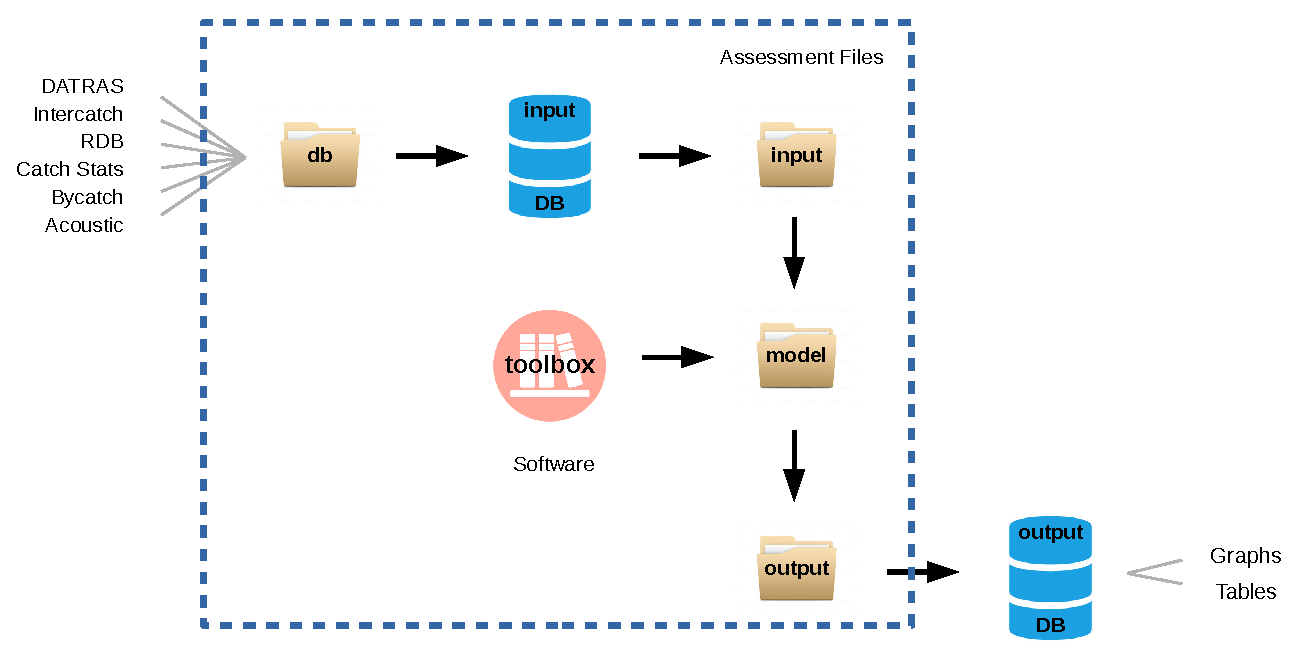
\includegraphics[width=0.8\textwidth]{taf-diagram}\\[-27.5ex]
  \onslide<+->
  \hspace{-14ex}
\includegraphics[width=0.58\textwidth]{taf-rollercoaster}
\end{frame}

% ______________________________________________________________________________

\begin{frame}{Example}{North Sea haddock}
  \centering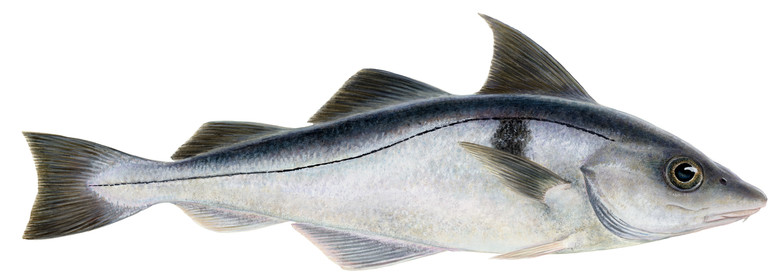
\includegraphics{haddock}\\[-13ex]
  \hspace{40ex}{\footnotesize\green yay, data!}\\[13ex]
\end{frame}

% ______________________________________________________________________________

\begin{frame}{DATRAS}{click-click interface}
  \vspace{-4ex}
  \begin{center}
    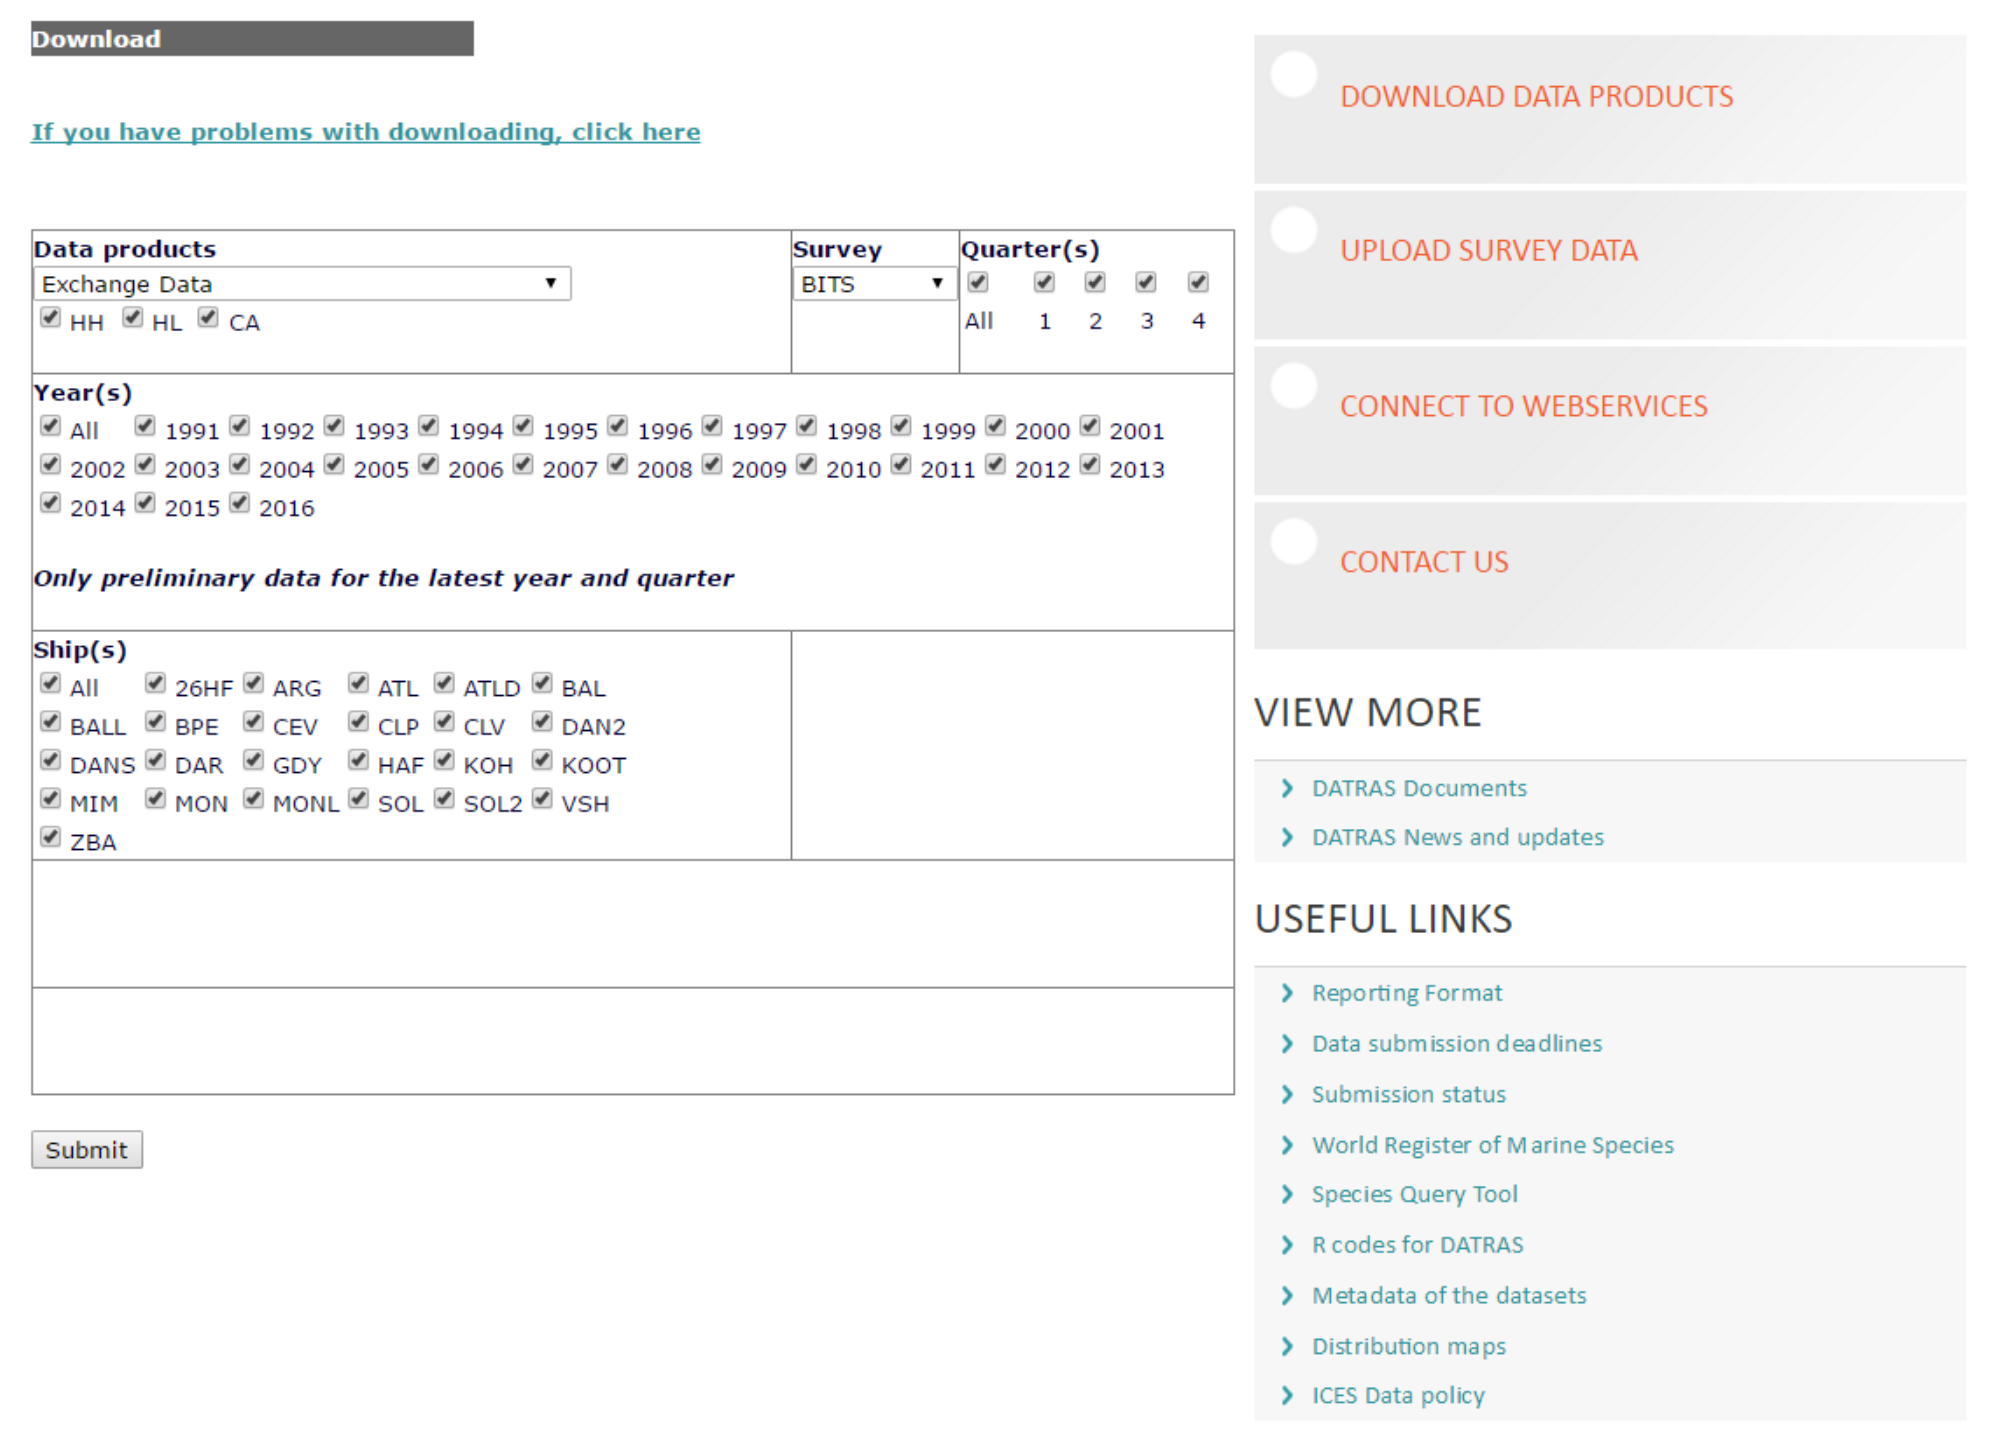
\includegraphics[height=0.75\textheight]{datras-click}
  \end{center}
  \vspace{-7ex}
  \quad\small\orange Not useful for scripting...\\[4ex]
\end{frame}

% ______________________________________________________________________________

\begin{frame}{DATRAS}{web service}
  \begin{columns}
    \column{0.4\textwidth}\scriptsize
    \footnotesize The following operations are supported:\\[-0.5ex]
    \begin{enumerate}[-]\blue
      \item getCAdata\\[-1ex]
      \item getHHdata\\[-1ex]
      \item getHLdata\\[-1ex]
      \item getSurveyInsertDate\\[-1ex]
      \item getSurveyList\\[-1ex]
      \item getSurveyYearList\\[-1ex]
      \item getSurveyYearQuarterList\\[-1ex]
    \end{enumerate}
    \column{0.5\textwidth}
    \vspace{1ex}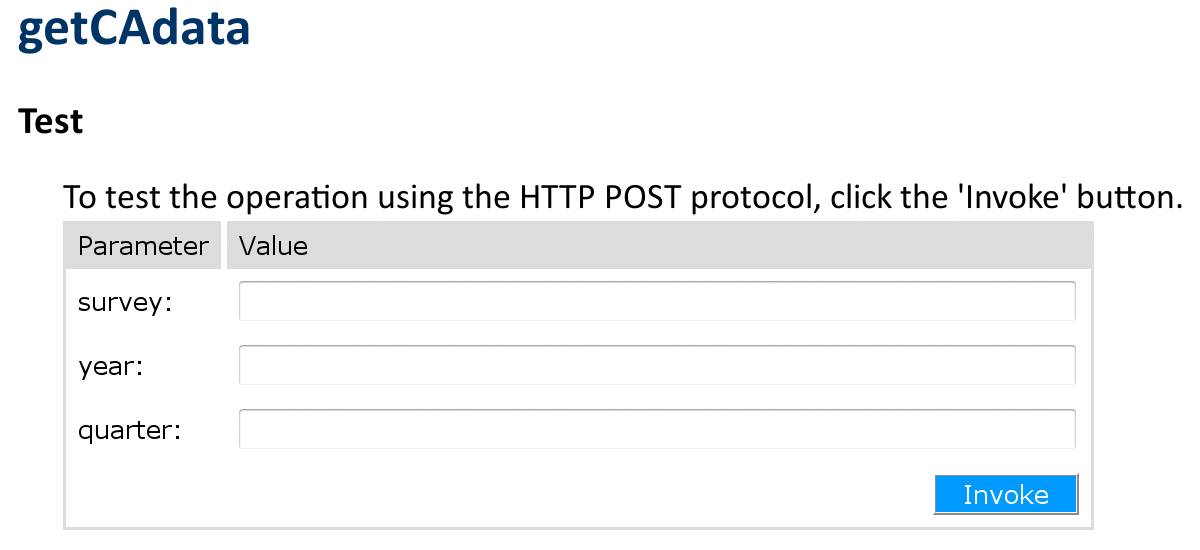
\includegraphics[width=\textwidth]{datras-getca}
  \end{columns}
  \vspace{5ex}\footnotesize
  {\green URL to get NS-IBTS survey data from 1965, quarter 1:}\\[2ex]
  \hspace{3.6ex}
  \begin{minipage}{60ex}
    \setlength\parindent{-15pt}
    \scriptsize\url{https://datras.ices.dk/WebServices/DATRASWebService.asmx/getCAdata?survey=NS-IBTS\&year=1965\&quarter=1}
  \end{minipage}
\end{frame}

% ______________________________________________________________________________

% ______________________________________________________________________________

\begin{frame}{Data formats}
  \begin{itemize}
    \item[-] XML, POX
    \item[-] JSON
    \item[-] CSV
  \end{itemize}
\end{frame}

% \begin{frame}{Data formats}
%   \textbf{DATRAS}\\
%   \begin{minipage}{60ex}
%     \setlength\parindent{-15pt}
%     \blue\scriptsize\url{https://datras.ices.dk/WebServices/DATRASWebService.asmx/getCAdata?survey=NS-IBTS\&year=1965\&quarter=1}
%   \end{minipage}\\
%   \textbf{SAG}\\

%   \textbf{SLD}\\
%   \blue\scriptsize\url{http://stocklist.ices.dk/services/odata4/StockListDWs4}
% \end{frame}

% ______________________________________________________________________________

\begin{frame}{Using web services in R}\small
  \begin{enumerate}
    \item Construct URL of interest\\[0.5ex]
    \begin{itemize}\item[]
      \begin{minipage}{60ex}
        \setlength\parindent{-15pt}
        \scriptsize\blue\url{https://datras.ices.dk/WebServices/DATRASWebService.asmx/getCAdata?survey=NS-IBTS\&year=1965\&quarter=1}\\[3ex]
      \end{minipage}
    \end{itemize}
    \item Send URL, read data object\\[6ex]
    \item Convert object to data frame\\[0.5ex]
    \quad\gray\footnotesize ... unless it already is a data frame\\[1ex]
  \end{enumerate}
\end{frame}

% ______________________________________________________________________________

\begin{frame}{icesDatras}{R package}\scriptsize
  \textgray{Description}\\[-1.5ex]
  \begin{itemize}
    \item[] R interface to access the web services of the ICES\\[0.2ex]
    (International Council for the Exploration of the Sea)\\[0.2ex]
    DATRAS trawl database.
  \end{itemize}
  \textgray{Details}\\[-1.5ex]
  \begin{itemize}
    \item[] \it\hspace{-1ex} Get dataset:
  \end{itemize}\vspace{-1.3ex}\hspace{6ex}
  \begin{tabular}{ll}
    \tt\r{getHHdata} & haul data        \\
    \tt\r{getHLdata} & length-based data\\
    \tt\r{getCAdata} & age-based data   \\
    \tt\r{getDATRAS} & any data         \\
  \end{tabular}\\[-1ex]
  \begin{itemize}
    \item[] \it\hspace{-1ex} Overview of available data:
  \end{itemize}\vspace{-1.3ex}\hspace{6ex}
  \begin{tabular}{ll}
    \tt\r{getSurveyList}            & surveys                     \\
    \tt\r{getSurveyYearList}        & years                       \\
    \tt\r{getSurveyYearQuarterList} & quarters                    \\
    \tt\r{getDatrasDataOverview}    & surveys, years, and quarters\\
  \end{tabular}\\[2ex]
  \textgray{Author(s)}\\[-1ex]
  \begin{itemize}
    \item[] Colin Millar, Einar Hjorleifsson, Scott Large, and Arni
    Magnusson\\[5ex]
  \end{itemize}
\end{frame}

% ______________________________________________________________________________

% \begin{frame}[fragile]{icesDatras}{R package}
% \begin{semiverbatim}
% \r{library}(icesDatras)
% getSurveyList()
% getSurveyYearList("NS-IBTS")
% getSurveyYearQuarterList("NS-IBTS", 1965)
% getCAdata("NS-IBTS", 1965, 1)
% getHHdata("NS-IBTS", 1965, 1)
% getHLdata("NS-IBTS", 1965, 1)
% getCatchWgt              function 22
% getDATRAS                function 30
% getDatrasDataOverview    function  9
% getHHdata                function  6
% getHLdata                function  6
% getSurveyList            function  3
% getSurveyYearList        function  4
% getSurveyYearQuarterList function  4
% \end{semiverbatim}
% \end{frame}

% ______________________________________________________________________________

\begin{frame}{R}
  Scientific data analysis, TAF\\[4ex]
  Interactive session, batch mode\\[4ex]
  Scripts, functions, packages
\end{frame}

% ______________________________________________________________________________

\begin{frame}{Reading data into R}
  Tabular text file (CSV)\\[4ex]
  XML\\[4ex]
  JSON\\[4ex]
\end{frame}

% ______________________________________________________________________________

\begin{frame}{ICES packages for web services}
  icesDatras\\[4ex]
  icesSAG\\[4ex]
  icesSLD\\[4ex]
  icesVocab
\end{frame}

% ______________________________________________________________________________

\begin{frame}{Handling unusual data}
  NA\\[4ex]
  Whitespace\\[4ex]
  International characters
\end{frame}

% ______________________________________________________________________________

\begin{frame}{Possible improvements}
  Select species from DATRAS, CSV format\\[4ex]
  Get survey indices (and other data products) from DATRAS into R\\[4ex]
  Commercial catch-at-age web services\\[4ex]
  [Data products could be provided using web service operators,\\[1ex]
  or R functions somewhere]
\end{frame}

\end{document}
